% ============================================================
% Informe: Heurísticas de eliminación en OpenMarkov
% ============================================================
\documentclass[11pt, a4paper]{article}

\usepackage[utf8]{inputenc}
\usepackage[T1]{fontenc}
\usepackage[spanish, es-nodecimaldot]{babel}
\addto\captionsspanish{\renewcommand{\tablename}{Tabla}}
\usepackage{geometry}
\geometry{margin=2.5cm}
\usepackage{amsmath}
\usepackage{amssymb}
\usepackage{booktabs}
\usepackage{array}
\usepackage{xcolor}
\usepackage{listings}
\usepackage{caption}
\usepackage{hyperref}
\usepackage{parskip}
\usepackage{graphicx}

% ---- código fuente ----
\lstset{
  language=Java,
  basicstyle=\ttfamily\small,
  keywordstyle=\color{blue!70!black}\bfseries,
  commentstyle=\color{gray},
  stringstyle=\color{orange!80!black},
  showstringspaces=false,
  breaklines=true,
  frame=single,
  framesep=4pt,
  xleftmargin=6pt,
  xrightmargin=6pt,
  tabsize=4,
  columns=flexible,
  numbers=left,
  numberstyle=\tiny\color{gray},
  numbersep=6pt,
  literate=
    {á}{{\'{a}}}1 {é}{{\'{e}}}1 {í}{{\'{i}}}1 {ó}{{\'{o}}}1 {ú}{{\'{u}}}1
    {Á}{{\'{A}}}1 {É}{{\'{E}}}1 {Í}{{\'{I}}}1 {Ó}{{\'{O}}}1 {Ú}{{\'{U}}}1
    {ñ}{{\~{n}}}1 {Ñ}{{\~{N}}}1 {ü}{{\"u}}1
}

% ============================================================
\title{Mejoras en las heurísticas de eliminación de variables\\
       de OpenMarkov}
\author{CISIAD --- UNED}
\date{Marzo 2026}

\begin{document}
\maketitle
\tableofcontents
\bigskip\bigskip

% ============================================================
\section{Introducción}

Las heurísticas de eliminación de variables determinan el orden en que se eliminan las variables al triangular el grafo moral de una red bayesiana. Un buen orden de eliminación minimiza el \emph{treewidth}, es decir, el tamaño del clique más grande generado durante la triangulación menos uno. Cuanto menor es el treewidth, menor es el coste de la inferencia exacta.

OpenMarkov proporciona varias heurísticas de eliminación. En este documento se describen tres grupos de cambios realizados:

\begin{enumerate}
  \item Corrección de dos errores en \texttt{CanoMoralElimination}.
  \item Implementación de una nueva heurística greedy: \texttt{WeightedMinFill}.
  \item Implementación de un marco genérico de búsqueda anticipada (\emph{lookahead}) y tres instancias concretas: \texttt{LookaheadMinFill}, \texttt{LookaheadMinCliqueSize} y \texttt{LookaheadCanoMoral}.
\end{enumerate}

% ============================================================
\section{Corrección de \texttt{CanoMoralElimination}}
\label{sec:canomoral}

La clase \texttt{CanoMoralElimination} implementa el algoritmo de triangulación heurística de Cano y Moral~\cite{CanoMoral1991}. La métrica que utiliza es:

\begin{equation}
  H_6(X_i) = \frac{S(X_i)}{C(X_i)}
  \label{eq:h6}
\end{equation}

donde $S(X_i)$ es el tamaño del clique creado al eliminar $X_i$ (producto de las cardinalidades de $X_i$ y sus vecinos), y $C(X_i)$ es la suma de los tamaños de todos los cliques maximales del subgrafo inducido por $X_i$ y sus vecinos. Se elimina la variable con menor $H_6$.

Se detectaron dos errores independientes:

\subsection{Error 1: la lista de cliques maximales siempre estaba vacía}

En el método \texttt{sumCliqueSizes}, el bucle que evita añadir cliques ya subsumidos usaba la condición incorrecta:

\begin{lstlisting}[caption={Condición original (incorrecta)}]
for (i = 0; i < numMaximalCliques && !maximalCliques.get(i).containsAll(maximalClique); i++) { }
if (i < numMaximalCliques) {   // BUG: debería ser i == numMaximalCliques
    maximalCliques.add(maximalClique);
}
\end{lstlisting}

La condición \texttt{i < numMaximalCliques} es cierta cuando el bucle terminó \emph{antes de recorrer todos los cliques}, es decir, cuando encontró uno que sí subsume al nuevo. La condición \emph{correcta} para añadir el clique es que el bucle haya llegado al final sin encontrar ningún subsumisor:

\begin{lstlisting}[caption={Condición corregida}]
if (i == numMaximalCliques) {
    maximalCliques.add(maximalClique);
}
\end{lstlisting}

Como consecuencia del bug original, \texttt{sumCliqueSizes} siempre devolvía~0, lo que hacía que $H_6$ fuera siempre \texttt{MAX\_VALUE} para todos los nodos, y la heurística siempre elegía el último candidato de la lista (comportamiento arbitrario).

\subsection{Error 2: \texttt{getMaxClique} podía devolver \texttt{null}}

El método \texttt{getMaxClique} calcula el clique maximal que contiene una semilla dada. Su variable local \texttt{maxClique} se inicializaba a \texttt{null}:

\begin{lstlisting}[caption={Inicialización original (incorrecta)}]
Set<Node> maxClique = null;
long maxCliqueSize = 0;
for (Node node : candidates) {
    ...
    if (maxCliqueCandidateSize > maxCliqueSize) {
        maxClique = maxCliqueCandidate;
    }
}
return maxClique;  // devuelve null si candidates estaba vacío
\end{lstlisting}

Cuando no había ningún candidato para expandir la semilla (la semilla ya es un clique maximal), el método devolvía \texttt{null}. Esto provocaba una \texttt{NullPointerException} en \texttt{sumCliqueSizes} al comparar con \texttt{containsAll}. La corrección es inicializar \texttt{maxClique} con la semilla misma, que es el clique maximal cuando no existe ninguna expansión posible:

\begin{lstlisting}[caption={Inicialización corregida}]
Set<Node> maxClique = seed;
long maxCliqueSize = getCliqueSize(seed);
\end{lstlisting}

Los dos bugs eran independientes pero se enmascaraban mutuamente: mientras existió el primer bug, \texttt{getMaxClique} nunca era llamado desde \texttt{sumCliqueSizes} con una semilla que requiriera regresar \texttt{null}, por lo que el segundo bug no se manifestaba. Al corregir el primero, el segundo quedó expuesto.

% ============================================================
\section{Nueva heurística: \texttt{WeightedMinFill}}
\label{sec:wmf}

\subsection{Motivación}

La heurística \texttt{MinimalFillIn} cuenta el número de arcos de relleno (\emph{fill-in}) que generaría la eliminación de una variable, sin tener en cuenta el tamaño de las tablas de probabilidad asociadas a esas variables. \texttt{WeightedMinFill} corrige este sesgo ponderando cada arco de relleno por las cardinalidades de los dos extremos del arco.

\subsection{Función de coste}

Para una variable $X$ con vecinos $\mathcal{N}(X)$:

\begin{equation}
  \mathrm{cost}(X) = \sum_{\substack{Y, Z \in \mathcal{N}(X) \\ Y \neq Z \\ (Y,Z) \notin E}} \mathrm{card}(Y) \cdot \mathrm{card}(Z)
  \label{eq:wmf}
\end{equation}

donde la suma recorre todos los pares de vecinos de $X$ que \emph{no} están ya conectados por un arco (los que formarían arcos de relleno al eliminar $X$), y $\mathrm{card}(V)$ es el número de estados de la variable $V$.

\subsection{Criterio de desempate}

En caso de empate en el coste, se da prioridad a la variable con \emph{menos vecinos actuales}; si persiste el empate, se elige la variable de menor nombre (orden lexicográfico, tolerante a \texttt{null}).

\subsection{Implementación}

La clase extiende \texttt{EliminationHeuristic} y mantiene una copia del grafo (\texttt{graphCopy}) actualizada tras cada eliminación:

\begin{itemize}
  \item \texttt{getVariableToDelete()}: recorre los candidatos, calcula la ecuación~\eqref{eq:wmf} para cada uno mediante \texttt{weightedFillInCost(Node)} y devuelve el de menor coste.
  \item \texttt{afterEditExecutes(PNEdit)}: añade los arcos de relleno en \texttt{graphCopy} y elimina el nodo correspondiente.
\end{itemize}

% ============================================================
\section{Heurísticas con búsqueda anticipada (\emph{lookahead})}
\label{sec:lookahead}

\subsection{Motivación}

Las heurísticas greedy toman decisiones de eliminación mirando únicamente el coste inmediato. Una estrategia de búsqueda anticipada evalúa también las consecuencias de esa elección en pasos futuros, con la esperanza de evitar decisiones localmente buenas pero globalmente costosas.

\subsection{Algoritmo}

Sea $G$ el grafo moral actual, $X$ un candidato a eliminar y $d$ la profundidad de búsqueda. La función de puntuación es:

\begin{equation}
  \mathrm{score}(G, X, d) =
  \begin{cases}
    c_0(G, X)                                                                    & \text{si } d = 0 \\
    c_0(G, X) + \displaystyle\min_{Y \in \mathrm{beam}(G \setminus X)}\,\mathrm{score}(G \setminus X, Y, d-1) & \text{si } d > 0
  \end{cases}
  \label{eq:score}
\end{equation}

donde:
\begin{itemize}
  \item $c_0(G, X)$ es el \emph{coste inmediato} de eliminar $X$ (definido por la subclase concreta),
  \item $G \setminus X$ denota el grafo resultante de eliminar $X$ y añadir los arcos de relleno necesarios,
  \item $\mathrm{beam}(G')$ es el subconjunto de hasta \texttt{beamWidth} candidatos de menor coste inmediato en $G'$ (búsqueda en haz).
\end{itemize}

Los valores por defecto son \texttt{depth} $= 2$ y \texttt{beamWidth} $= 3$.

\subsection{Clase base: \texttt{LookaheadHeuristic}}

Para evitar la duplicación de código, se diseñó una clase abstracta \texttt{LookaheadHeuristic} que implementa toda la infraestructura del algoritmo~\eqref{eq:score}. Las subclases solo tienen que implementar:

\begin{lstlisting}[caption={Método plantilla de LookaheadHeuristic}]
protected abstract double immediateCost(boolean[][] adj, boolean[] active,
                                        int x, int[] cardinalities);
\end{lstlisting}

donde:
\begin{itemize}
  \item \texttt{adj}: la matriz de adyacencia actual (no se muta),
  \item \texttt{active}: máscara booleana de los nodos aún presentes,
  \item \texttt{x}: índice del nodo a evaluar,
  \item \texttt{cardinalities}: número de estados de cada nodo.
\end{itemize}

La búsqueda anticipada opera exclusivamente sobre una matriz \texttt{boolean[][]} ligera, sin construir copias de \texttt{ProbNet}. Esto hace que el coste adicional sea manejable. La copia real del grafo (\texttt{graphCopy}) solo se actualiza en \texttt{afterEditExecutes}, es decir, una vez por eliminación real, no durante la búsqueda.

\subsection{\texttt{LookaheadMinFill}}

Coste inmediato: fill-in ponderado (ecuación~\eqref{eq:wmf}), calculado directamente sobre la matriz booleana.

\begin{equation}
  c_0^{\mathrm{LMF}}(G, X) = \sum_{\substack{Y, Z \in \mathcal{N}(X) \\ (Y,Z) \notin E}} \mathrm{card}(Y) \cdot \mathrm{card}(Z)
\end{equation}

\subsection{\texttt{LookaheadMinCliqueSize}}

Coste inmediato: tamaño del clique que formaría $X$ con sus vecinos.

\begin{equation}
  c_0^{\mathrm{LCS}}(G, X) = |\mathcal{N}(X)| + 1
\end{equation}

\subsection{\texttt{LookaheadCanoMoral}}

Coste inmediato: la misma métrica $H_6$ de la ecuación~\eqref{eq:h6}, reimplementada sobre la representación \texttt{boolean[][]}. El método \texttt{getMaxClique} trabaja sobre máscaras booleanas en lugar de conjuntos de \texttt{Node}, con la misma lógica recursiva que en \texttt{CanoMoralElimination} pero sin dependencias de objetos del dominio.

\begin{equation}
  c_0^{\mathrm{LCM}}(G, X) = \frac{S(X)}{C(X)}
  \qquad \text{(cf. ecuación~\eqref{eq:h6})}
\end{equation}

% ============================================================
\section{Evaluación experimental}
\label{sec:eval}

\subsection{Alcance del experimento}

La heurística \texttt{LookaheadCanoMoral} no se incluye en la comparación experimental. Su función de coste inmediato requiere encontrar cliques maximales en el subgrafo de vecinos mediante un algoritmo recursivo (\texttt{getMaxClique}), cuyo coste crece exponencialmente con el número de vecinos. En redes grandes, el tiempo de evaluación hace que la heurística no termine en un plazo razonable. Las demás siete heurísticas sí se comparan.

\subsection{Metodología}

Se comparan las siete heurísticas sobre las redes bayesianas disponibles en el repositorio de OpenMarkov, filtradas para incluir solo redes con potenciales de tipo tabla y excluyendo las versiones con sufijo \texttt{-1-0} (que son duplicadas). El repositorio contiene actualmente 7 redes válidas tras aplicar estos filtros. Para cada par (red, heurística):

\begin{itemize}
  \item Se construye el árbol de unión mediante \texttt{HuginForest}.
  \item Se registran el \emph{treewidth} ($= \max_c |c| - 1$, donde $|c|$ es el número de variables del clique $c$) y la \emph{suma del árbol de unión} ($= \sum_c \prod_{V \in c} \mathrm{card}(V)$), que es el coste real de la inferencia.
  \item El tiempo máximo por par es 5~minutos. Si se supera, se registra \textsc{timeout}.
\end{itemize}

La ejecución se paraleliza usando un pool de \texttt{Runtime.getRuntime().\allowbreak availableProcessors()} hilos. La estrategia es fila a fila: las $H$ heurísticas de una misma red se ejecutan en paralelo; los resultados se recogen antes de cargar la siguiente red. Así el pico de memoria se limita a $H$ copias de una red en lugar de $N \times H$ simultáneas.

% ---- Tabla treewidth ----
\begin{table}[!htbp]
\centering
\renewcommand{\arraystretch}{1.15}
\resizebox{\linewidth}{!}{%
\begin{tabular}{lc *{7}{r}}
\toprule
\textbf{Red} & \textbf{Vars}
  & \textbf{SimpleElim}
  & \textbf{MinFillIn}
  & \textbf{MinClique}
  & \textbf{CanoMoral}
  & \textbf{WgtMinFill}
  & \textbf{LAMinFill}
  & \textbf{LAMinClique} \\
\midrule
BN-nasonet.pgmx           & 111 & 12 & 7 & 5 & \textbf{4} & 7 & 7 & 5 \\
BN-hepar.pgmx             &  71 & 17 & 5 & 5 & 6          & 5 & 6 & 6 \\
BN-prostanet.pgmx         &  47 & 12 & 4 & 4 & 5          & 5 & 5 & \textbf{4} \\
BN-alarm.pgmx             &  37 &  3 & \textbf{2} & \textbf{2} & 3 & \textbf{2} & \textbf{2} & \textbf{2} \\
BN-asia.pgmx              &   8 &  2 & 2 & 2 & 2          & 2 & 2 & 2 \\
BN-two-diseases-naive.pgmx &  8 & \textbf{1} & \textbf{1} & \textbf{1} & 4 & \textbf{1} & \textbf{1} & \textbf{1} \\
BN-one-disease.pgmx       &   2 &  1 & 1 & 1 & 1          & 1 & 1 & 1 \\
\bottomrule
\end{tabular}}
\caption{Treewidth obtenido por cada heurística sobre las redes bayesianas
         del repositorio (versiones canónicas; valor más bajo es mejor).
         En negrita el mejor resultado de cada fila.}
\label{tab:treewidth}
\end{table}

% ---- Tabla suma ----
\begin{table}[!htbp]
\centering
\renewcommand{\arraystretch}{1.15}
\resizebox{\linewidth}{!}{%
\begin{tabular}{lc *{7}{r}}
\toprule
\textbf{Red} & \textbf{Vars}
  & \textbf{SimpleElim}
  & \textbf{MinFillIn}
  & \textbf{MinClique}
  & \textbf{CanoMoral}
  & \textbf{WgtMinFill}
  & \textbf{LAMinFill}
  & \textbf{LAMinClique} \\
\midrule
BN-nasonet.pgmx           & 111 & 78.53M & 109.6K & 33.3K & \textbf{18.6K} & 163.9K & 98.5K & 34.3K \\
BN-hepar.pgmx             &  71 & 28.47M & 713 & 680 & 1\,500 & 692 & \textbf{628} & 640 \\
BN-prostanet.pgmx         &  47 & 40.6K  & \textbf{296} & 310 & 620 & 436 & 436 & 352 \\
BN-alarm.pgmx             &  37 & 508    & 404 & 343 & 669 & \textbf{232} & 358 & 377 \\
BN-asia.pgmx              &   8 & 32     & 32  & 32  & 32  & 32  & 32  & 32  \\
BN-two-diseases-naive.pgmx &  8 & \textbf{42} & \textbf{42} & \textbf{42} & 66 & \textbf{42} & \textbf{42} & \textbf{42} \\
BN-one-disease.pgmx       &   2 & 4      & 4   & 4   & 4   & 4   & 4   & 4   \\
\bottomrule
\end{tabular}}
\caption{Suma del árbol de unión (producto de cardinalidades de cada clique
         sumado sobre todos los cliques). Mide el coste real de la inferencia.
         Valores en miles (K) o millones (M) cuando corresponde.
         En negrita el mejor resultado de cada fila.}
\label{tab:sum}
\end{table}

\subsection{Análisis de resultados}

Las redes del repositorio son relativamente pequeñas (8--111 variables); los resultados deben interpretarse con esa cautela.

\paragraph{Treewidth.}
\texttt{CanoMoral} obtiene el menor treewidth en la red más grande (nasonet, 111 variables: treewidth~4 frente a~5 del siguiente). \texttt{LookaheadMinCliqueSize} es la única heurística lookahead que iguala ese resultado, y también es la mejor en prostanet. Sin embargo, \texttt{CanoMoral} se comporta de forma patológica en \texttt{BN-two-diseases-naive}: obtiene treewidth~4 mientras todas las demás obtienen~1. Esto sugiere que la métrica H6 tiene un caso desfavorable en redes con una topología determinada.

\paragraph{Suma del árbol de unión.}
Este indicador es más sensible a las diferencias. \texttt{CanoMoral} es la mejor en nasonet (18.6K frente a 33.3K de MinClique), pero la peor en alarm (669 frente a 232 de WeightedMinFill) y en two-diseases-naive (66 frente a 42 del resto). \texttt{WeightedMinFill} destaca como la mejor en alarm. \texttt{LookaheadMinFill} mejora a su versión greedy en hepar (628 frente a 713) pero queda por detrás en prostanet y alarm.

\paragraph{La búsqueda anticipada puede ser peor que su versión greedy.}
Esto se observa en hepar (LAMinClique $>$ MinClique para la suma) y alarm (ambas versiones lookahead superadas por WeightedMinFill). Las razones son:
\begin{enumerate}
  \item \textbf{Truncamiento del haz}: el haz de anchura~3 puede descartar buenos caminos.
  \item \textbf{Horizonte corto}: con profundidad~2, el algoritmo no ve el impacto más allá de dos pasos.
  \item \textbf{Objetivo inadecuado}: la función $\mathrm{score}$ minimiza la \emph{suma} de costes futuros, mientras que el treewidth depende del \emph{máximo} de los tamaños de clique.
  \item \textbf{Balance implícito}: las heurísticas greedy clásicas mantienen un reparto equilibrado de vecinos que la búsqueda anticipada puede romper.
\end{enumerate}

% ============================================================
\section{Diagrama de clases}
\label{sec:diagrama}

La figura~\ref{fig:clases} muestra la jerarquía de heurísticas de eliminación resultante. Las clases en naranja han sido corregidas; las clases en verde son nuevas heurísticas greedy; las clases en azul pertenecen al nuevo marco de búsqueda anticipada. El diagrama fue generado con PlantUML a partir de \texttt{diagrama\_clases.puml}.

\begin{figure}[!htbp]
\centering
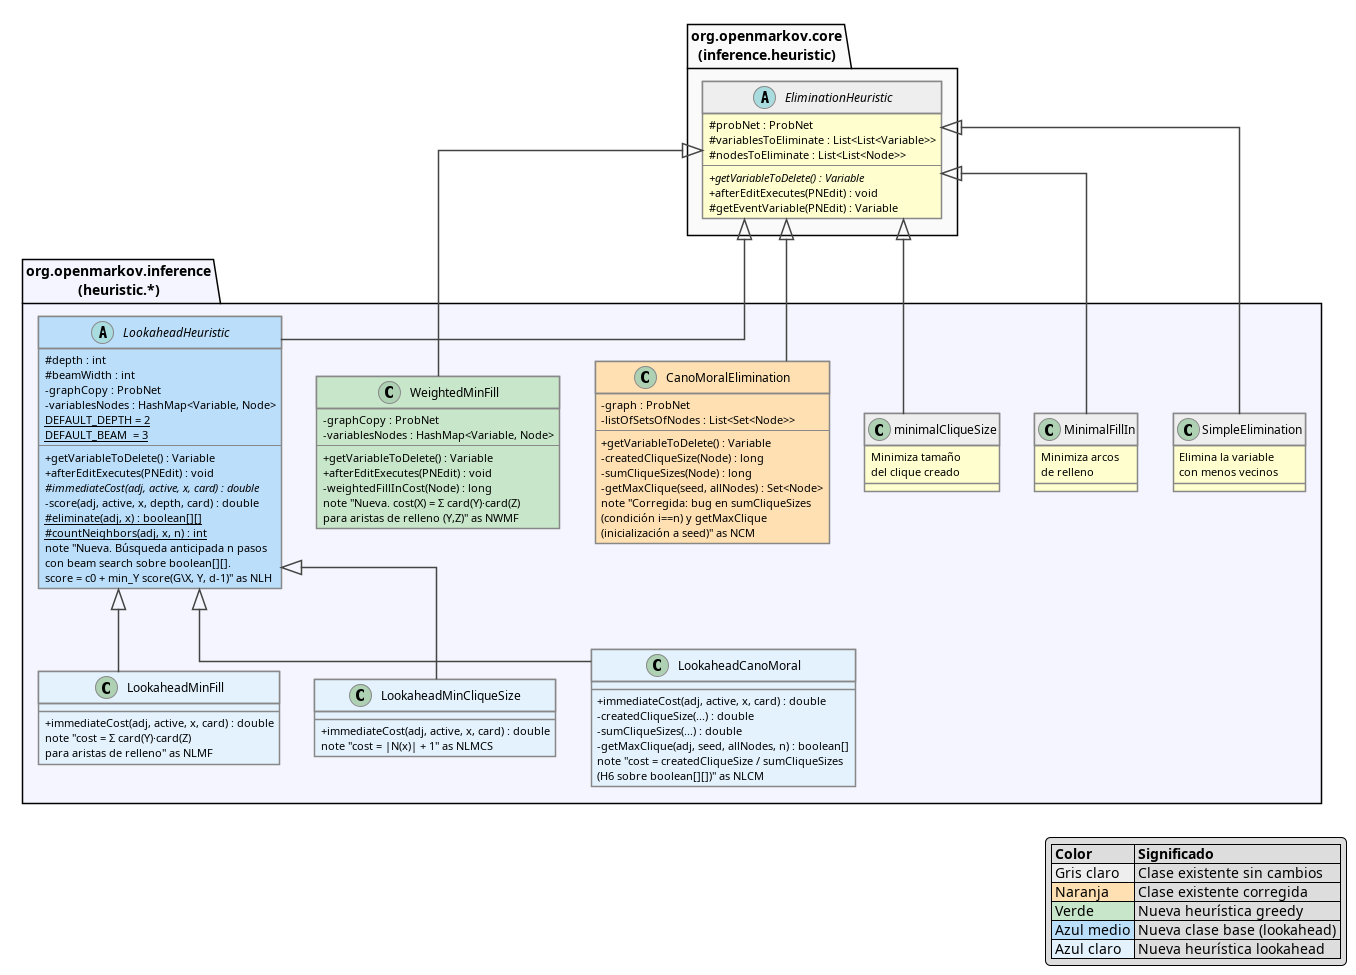
\includegraphics[width=\linewidth]{diagrama_clases}
\caption{Diagrama de clases de las heurísticas de eliminación de OpenMarkov
         tras las modificaciones descritas en este documento.}
\label{fig:clases}
\end{figure}

% ============================================================
\section{Resumen de ficheros modificados}
\label{sec:ficheros}

\begin{table}[h]
\centering
\caption{Ficheros afectados por los cambios descritos en este documento.}
\label{tab:ficheros}
\renewcommand{\arraystretch}{1.2}
\begin{tabular}{p{7.5cm} p{2.2cm} p{5cm}}
\toprule
\textbf{Fichero} & \textbf{Módulo} & \textbf{Cambio} \\
\midrule
\texttt{heuristic/canoAndMoral/CanoMoralElimination.java}
  & inference & Corrección de dos bugs \\
\texttt{heuristic/weightedMinFill/WeightedMinFill.java}
  & inference & Nueva clase \\
\texttt{heuristic/lookahead/LookaheadHeuristic.java}
  & inference & Nueva clase abstracta \\
\texttt{heuristic/lookahead/LookaheadMinFill.java}
  & inference & Nueva clase \\
\texttt{heuristic/lookahead/LookaheadMinCliqueSize.java}
  & inference & Nueva clase \\
\texttt{heuristic/lookahead/LookaheadCanoMoral.java}
  & inference & Nueva clase \\
\texttt{src/main/java/module-info.java}
  & inference & Exportación de paquetes nuevos \\
\texttt{inference/heuristics/HeuristicComparisonTest.java}
  & integrationtests & Test comparativo con paralelismo \\
\texttt{run-heuristic-comparison.sh}
  & (raíz) & Script de ejecución del test \\
\bottomrule
\end{tabular}
\end{table}

% ============================================================
\begin{thebibliography}{9}
\bibitem{CanoMoral1991}
A.~Cano y S.~Moral.
\newblock Heuristic algorithms for the triangulation of graphs.
\newblock En \emph{Proceedings of IPMU'94}, págs.~298--307, 1994.
\end{thebibliography}

\end{document}
